\subsection{System Architecture}
Our system architecture is designed with a thought-process of leveraging the power of containerization and using CouchDB with AURIN in the most efficient manner. The core components of the architecture are \texttt{Application} and \texttt{Harvester}, which are built into docker images and ran in their individual docker containers as shown in Figure \ref{fig:sysarchitecture}.

\begin{figure}[H]
    \centering
    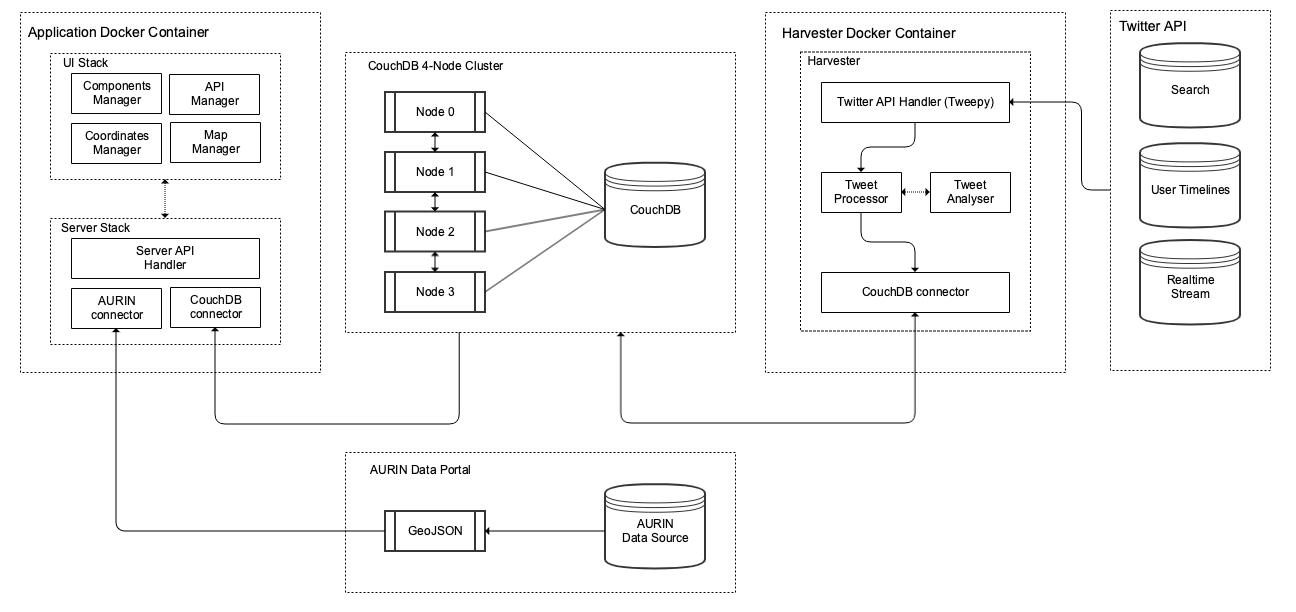
\includegraphics[width=16cm,keepaspectratio=true]{images/cloud_assignment_architecture.png}
    \caption{System Architecture Design}
    \label{fig:sysarchitecture}
\end{figure}

\textbf{Application.} This container provides the user-interface for interactions and operations. It is implemented with several modules which helps in providing seamless and intuitive experience.

\texttt{Components Manager.} This module is responsible for creating and styling all UI-related elements on the browser. It initializes basic UI classes and handle events of the HTML elements for seamless UX.

\texttt{API Manager.} This module provides interface for interacting with the server stack of the application. Using this manager, data and manipulation API request can be created and response delegated to the respective callbacks.

\texttt{Coordinates Manager.} This modules is responsible of providing coordinates related information and perform filtering if required.

\texttt{Map Manager.} All map related operations and manipulations are handled by this module. It uses other modules for its intuitive functioning using which it is able to plot tweets and AURIN data based on the events triggered by the user.

\texttt{Server API Handler.} This module is implemented on the server stack which is responsible of providing API endpoints on which UI stack can hit and extract data. It handles request and delegate it to appropriate function depending upon the resource requirements.

\texttt{AURIN connector.} This connector is implemented for providing interface for fetching data from GeoJSON extracted from AURIN data portal. This GeoJSON is saved inside the server stack and depending upon the dataset key requested, correct data is provided to the UI.

\texttt{CouchDB connector.} This connector is implemented for providing interface for fetching data from CouchDB. It has the capability of buffering data from couchdb depending upon the configurations provided.

\begin{figure}[H]
    \centering
    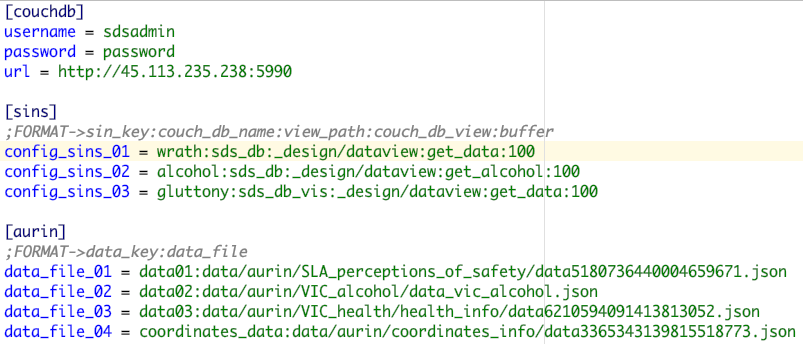
\includegraphics[width=12cm,keepaspectratio=true]{images/connector_config.png}
    \caption{Connectors configuration setup using \texttt{connectors.ini}}
    \label{fig:connectorconfig}
\end{figure}

\textbf{Harvester.} This container provides the tweet harvesting application, allowing for easy deployment and separation of dependencies.

\texttt{Twitter API handler.} This uses Tweepy to connect to the Twitter Search, real-time stream, and user timeline APIs. It handles authentication, rate limits, and request formats.

\texttt{Tweet processor.} The tweet processor is responsible for determining a) which tweets are relevant, and b) the locations from which tweets should be gathered. It stores all generally relevant tweets (i.e., tweets with locations in Melbourne) and story-relevant tweets in CouchDB via the CouchDB connection.

\texttt{Tweet analyser.} The analyzer determines whether a tweet is relevant to the story based on its text.

\texttt{CouchDB connector.} The CouchDB connector provides the layer through which the harvester accesses CouchDB, handling such things as creating and exposing individual databases.